\documentclass{article}
\usepackage{gensymb, amsmath, float, graphicx, epstopdf}
\restylefloat{table}
\usepackage[margin=0.75in]{geometry}
\begin{document}

\title{Lab Write-up 2: The Smith Chart}
\author{Michael Shen}
\maketitle


\section{Line Parameters of a Lossless Line}

\subsection{Measured Data}

\begin{table}[h]
\centering
	\begin{tabular}{rl}
	Patch Cord Length =  	  & 0.6229 $m$  \\
	Added Electrical Delay =  & 6.2565 $ns$      
	\end{tabular}
\end{table}

\subsection{Analysis}

\begin{enumerate}
	\item 
		\begin{equation}
			u_p = \dfrac{2l}{\Delta t}
		\end{equation}
		Using the measured data and Eq. 1, the calculated $u_p$ is $1.99\times 10^8$ $m/s$
	\item
		\begin{equation}
			\sqrt{\varepsilon_r} = \dfrac{c}{u_p}
		\end{equation}
		Using the result from problem 1 and Eq. 2, the calculated $\varepsilon_r$ is 2.270.
	\item
		\begin{equation}
			\beta = 2\pi f\sqrt{\mu\varepsilon}
		\end{equation}
		\begin{equation}
			\varepsilon = \varepsilon_0\varepsilon_r
		\end{equation}
		Using the result from problem 2, Eq. 3 and 4, $\varepsilon_0 = 8.85\times 10^{-12}$ $F/m$ and $\mu = \mu_0 = 4\pi\times 10^-7$ $H/m$, the calculated $\beta$ is $25.256$.
	\item
		\begin{equation}
			\begin{cases} 
				Z_0 = \sqrt{\dfrac{L}{C}} \\
				\sqrt{\mu\varepsilon} = \sqrt{LC}
			\end{cases}
		\end{equation}
		Since $Z_0 = 50 \Omega$, solving the system of equations results in $C = 1.00\times 10^{-10}$ $F$ and $L = 2.51\times 10^{-7}$ $H$.		
		
\end{enumerate}

\subsection{Questions}

\begin{enumerate}
	\item The line was assumed to be lossless, so $R'$ and $G'$ are both 0.
	\item A dispersionless line ensures that $u_p$ is not frequency dependent, that is, all waves travel at the same $u_p$. Lossless lines ensure that there is no power loss along the line. We could use this technique to measure the line parameters for a dispersionless line because $u_p$ will be a constant.
	\item I would not be able to obtain any useful data by analyzing a matched load by adding electrical delay. This is because a matched load completely absorbs a signal, reflecting nothing back, regardless of any phase shift.
	\item The time delay is added onto the time it takes for the signal to travel down to the shorted termination and back, thus we must use the fact that it travels the length of the cable twice when computing $u_p$.
\end{enumerate}


\section{Lossy and Lossless Lines on the Smith Chart}

\subsection{Analysis}
\begin{enumerate}
	\item The display appears to be a couple of overlapping circles with a constant $\vert\Gamma\vert\approx 1$. They are relatively stationary in their position on the Smith Chart, with no spiral pattern.
	\item The display appears to be a pattern spiralling inwards with $\vert\Gamma\vert$ starting around 0.5 and constantly decreasing as the frequency increases. This is because the line is lossy, which means some power is absorbed by the line. Thus, by electrically increasing the length of the line, more and more power will be absorbed by the line, reducing the amount of reflected power and $\vert\Gamma\vert$
\end{enumerate}

\subsection{Questions}
\begin{enumerate}
	\item If a lossy line is infinite in length, any power sent down the line would be absorbed by the line, that is, no power would be reflected back. Using Eq. 6, 
	\begin{equation}
		P_{av}^r = -\vert\Gamma\vert^2 \frac{\vert V_0^+\vert^2}{2Z_0}
	\end{equation}
We can see that this means that $\Gamma$ = 0. Thus, the response should spiral to the origin of the Smith Chart.
\end{enumerate}


\section{Impedance Measurements Using the Smith Chart}

\subsection{Measured Data}
\begin{table}[H]
\centering
	\begin{tabular}{rl}
	Resistor =   & 10 $\Omega$  \\
	Capacitor =  & 39 $pF$      
	\end{tabular}
\end{table}

\begin{table}[H]
\centering
\begin{tabular}{|l|l|l|l|l|}
\hline
\multicolumn{1}{|c|}{\textbf{Load}} & \multicolumn{1}{c|}{\textbf{400 MHz}} & \multicolumn{1}{c|}{\textbf{600 MHz}} & \multicolumn{1}{c|}{\textbf{800 MHz}} & \multicolumn{1}{c|}{\textbf{1.0 GHz}} \\ \hline
Short                               & 0.06031 + j2.208                      & 0.07049 + j3.2748                     & 0.1680 + j4.621                       & 0.01835 + j5.789                      \\ \hline
Open                                & 51.12 - j927.1                        & -16.49 - j713.9                       & -3.485 - j483.5                       & 8.908 - j304.2                        \\ \hline
Resistive                           & 11.57 + j19.34                        & 14.05 + j31.05                        & 18.65 + j45.98                        & 28.90 + j66.99                        \\ \hline
Capacitive                          & 2.895 - j750.6                        & 1.832 - j524.7                        & -2.166 - j377.4                       & 10.91 - j293.2                        \\ \hline
Series                              & 11.10 + j11.26                        & 14.76 + j28.21                        & 23.72 + j50.55                        & 52.46 + j88.62                        \\ \hline
Parallel                            & 5.481 + j12.63                        & 2.812 + j23.19                        & 1.168 + j35.15                        & 341.0 + j48.125
\\ \hline
\end{tabular}
	\caption{Voltage and phase measurements for varying signal frequency and cable length}
	\label{Data 1}
\end{table}

\subsection{Analysis}

\begin{enumerate}
	\item
	\item
	\item
	\item
\end{enumerate}

\subsection{Questions}

\begin{enumerate}
	\item A short termination has $\Gamma$ = 1, while an open termination has $\Gamma$ = -1. These are represented on opposite sides of the Smith Chart. Therefore, to make a short appear as if it were an open, the transmission line would need to be $\frac{\lambda}{2}$ long. The actual length is frequency dependent because $\lambda = \frac{u_p}{f}$.
	\item
\end{enumerate}


\section{Impedance Matching Using a Single Stub Tuner}

\subsection{Measured Data}

\begin{table}[H]
\centering
	\begin{tabular}{rl}
	Impedance before Matching =   			 & 23.79 + j63.00 $\Omega$  \\
	Distance between Load and Stub Tuner =   & 2.54 $cm$  \\
	Length of Stub =   						 & 11.2713 $cm$  \\
	Impedance after Matching =  			 & 185.5 - j11.54 $\Omega$      
	\end{tabular}
\end{table}

\subsection{Analysis}

\begin{enumerate}
	\item
	\item
	\item
\end{enumerate}

\subsection{Questions}

\begin{enumerate}
	\item No, I was unable to achieve a perfect match with the single stub tuner because a perfect match requires two degrees of freedom, the length of the stub and the distance from the stub to the load, to match the real and imaginary parts of the impedance. I only had the ability to change one, the length of the stub. This allows me to negate the imaginary part of the impedance.
	\item No, a quarter-wavelength transformer will have the same issue. Since the impedance is complex, a perfect match would require the ability to choose where to place the quarter-wavelength transformer. I did not have this option in lab. However, it is possible that the quarter-wavelength transformer achieves a better match for the unknown load, but it is not guaranteed.
	\item By using both the single stub tuner and quarter-wavelength transformer in conjunction, a perfect match can be achieved. First, the single stub tuner's length can be adjusted such that the imaginary part of the impedance as seen from the source becomes zero. Then, a quarter wavelength transformer can be inserted between the source. The quarter-wavelength transformer must have a specific impedance, $Z_0$, calculated from Eq. XXX such that it allows the aggregate input impedance, $Z_{in}$, to be matched.
	\begin{equation}
		Z_{in} = \dfrac{Z_0^2}{Z_L}
	\end{equation}
\end{enumerate}


\section{Figures and Images}
\begin{figure}[H]
    \centering
    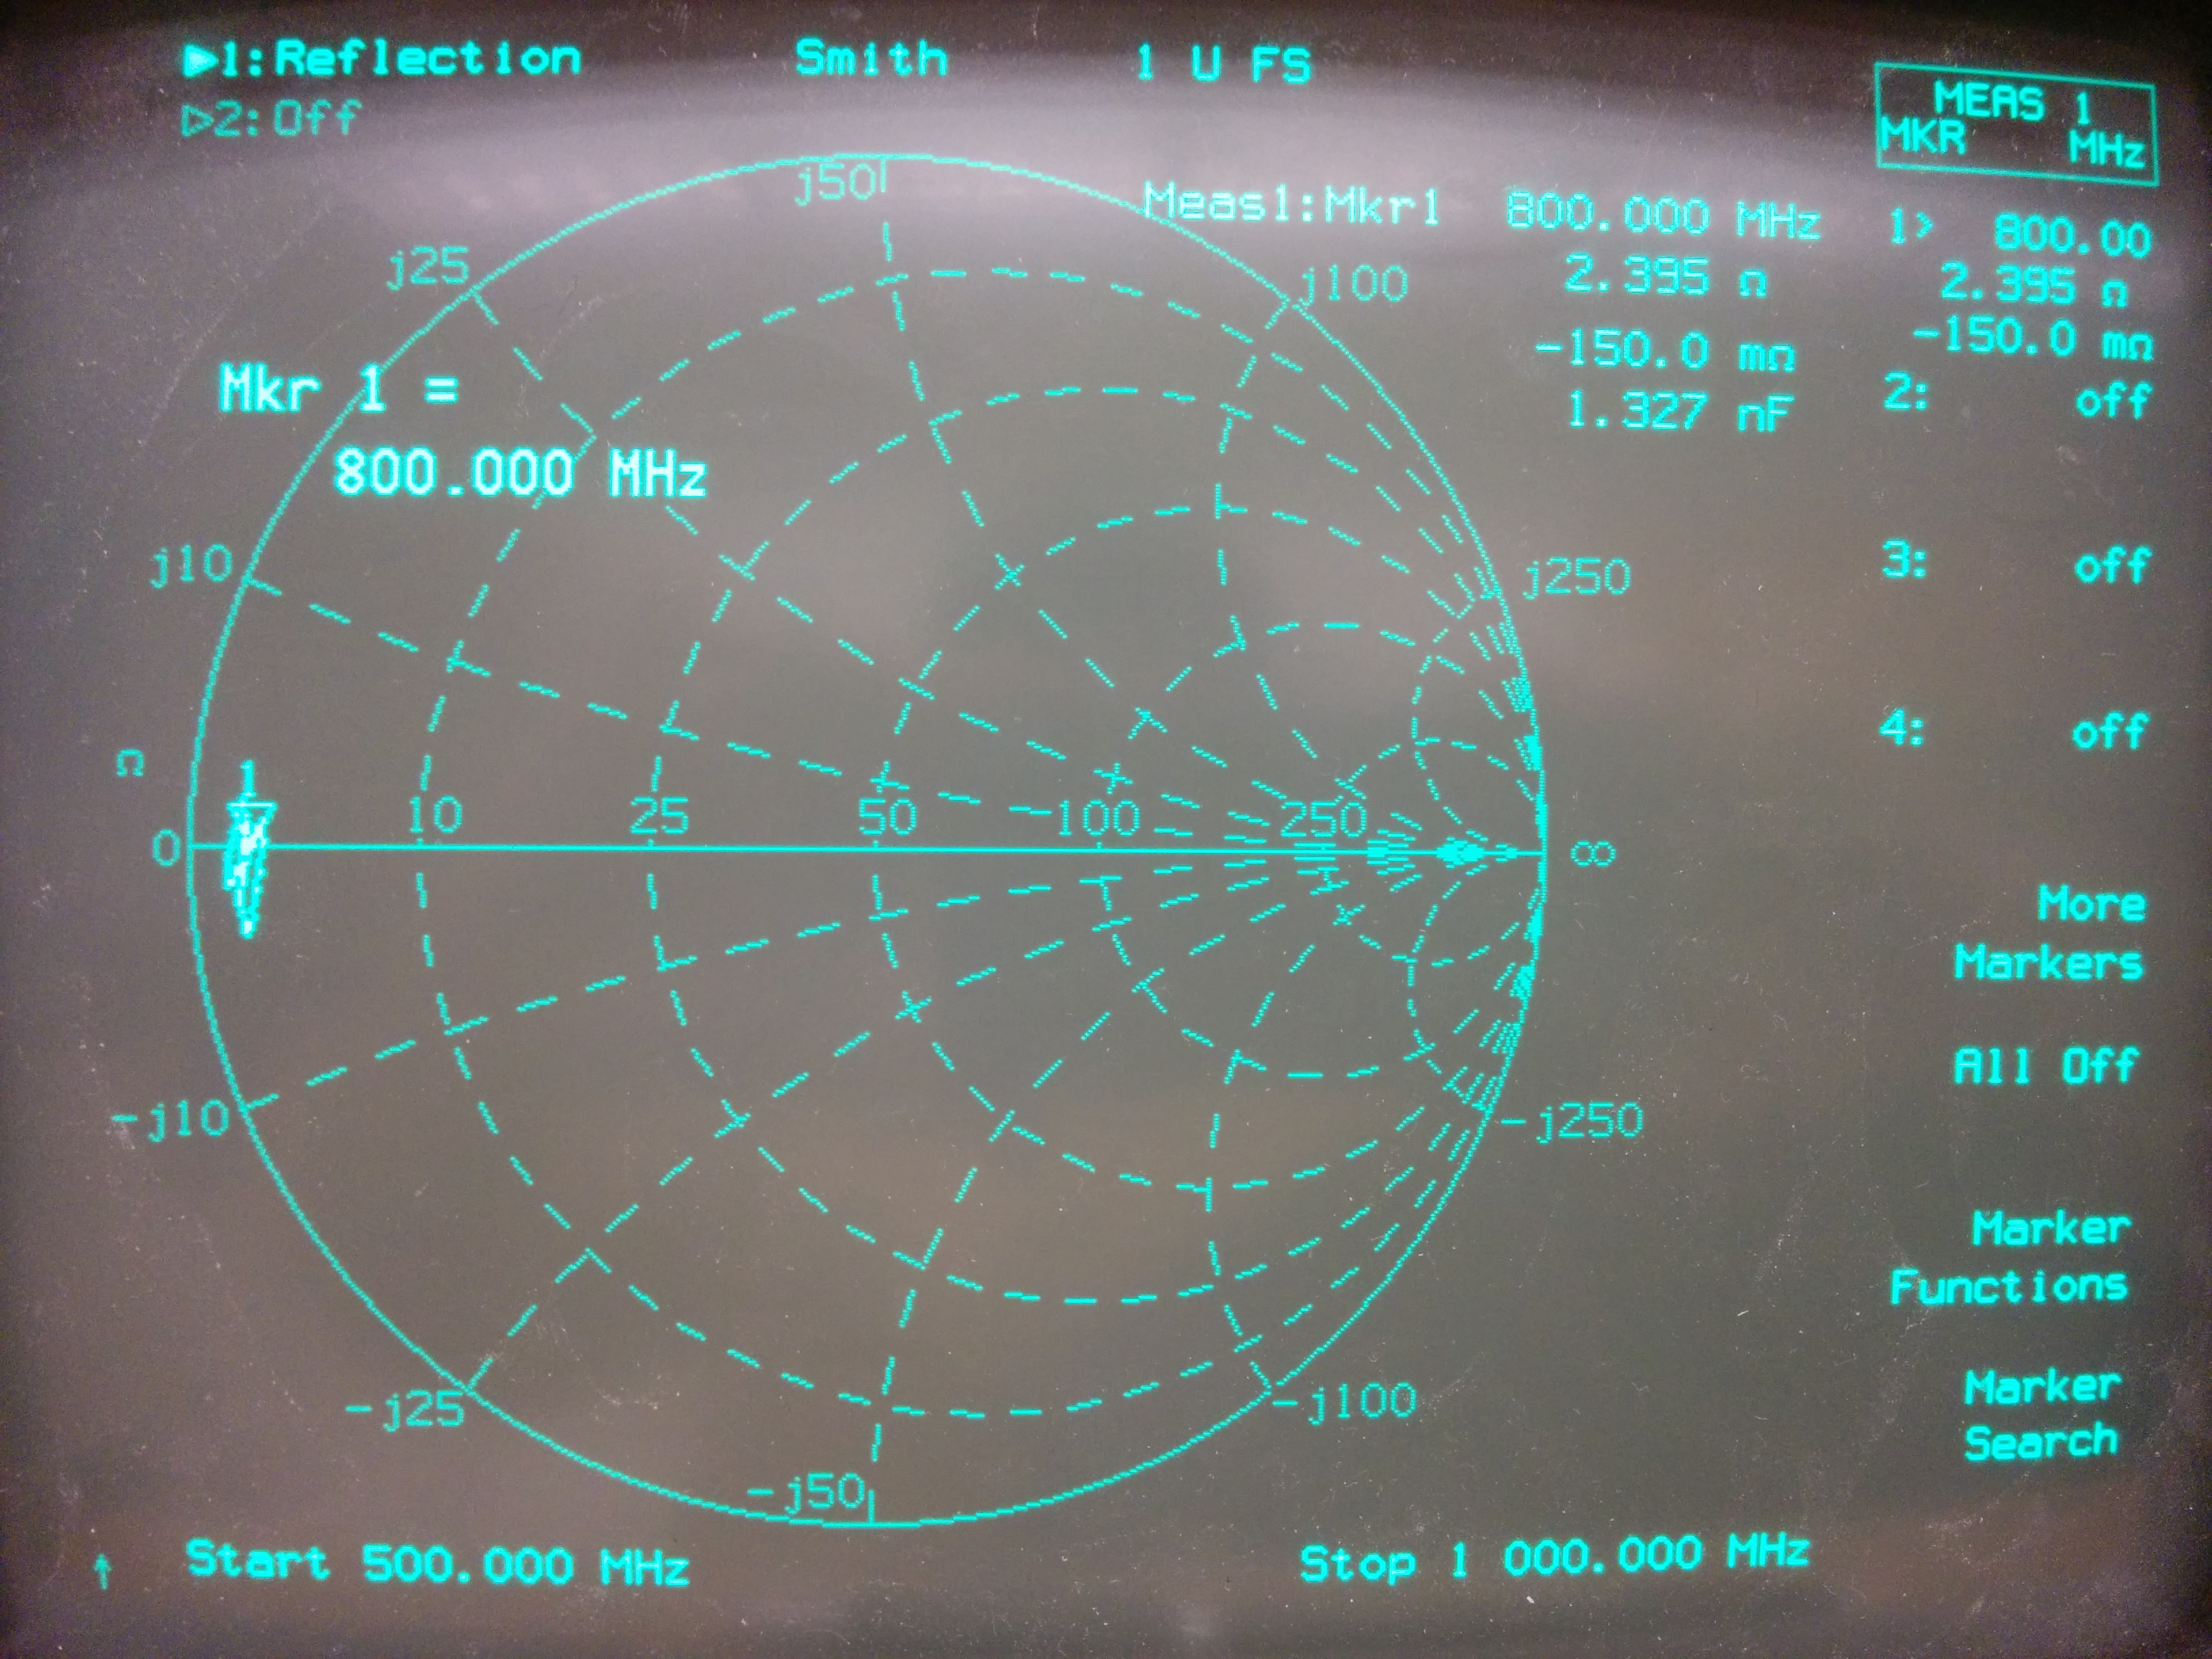
\includegraphics[width=0.8\textwidth]{./Images/251.jpg}
    \caption{Point-like response for a lossless line}
\end{figure}
\begin{figure}[H]
    \centering
    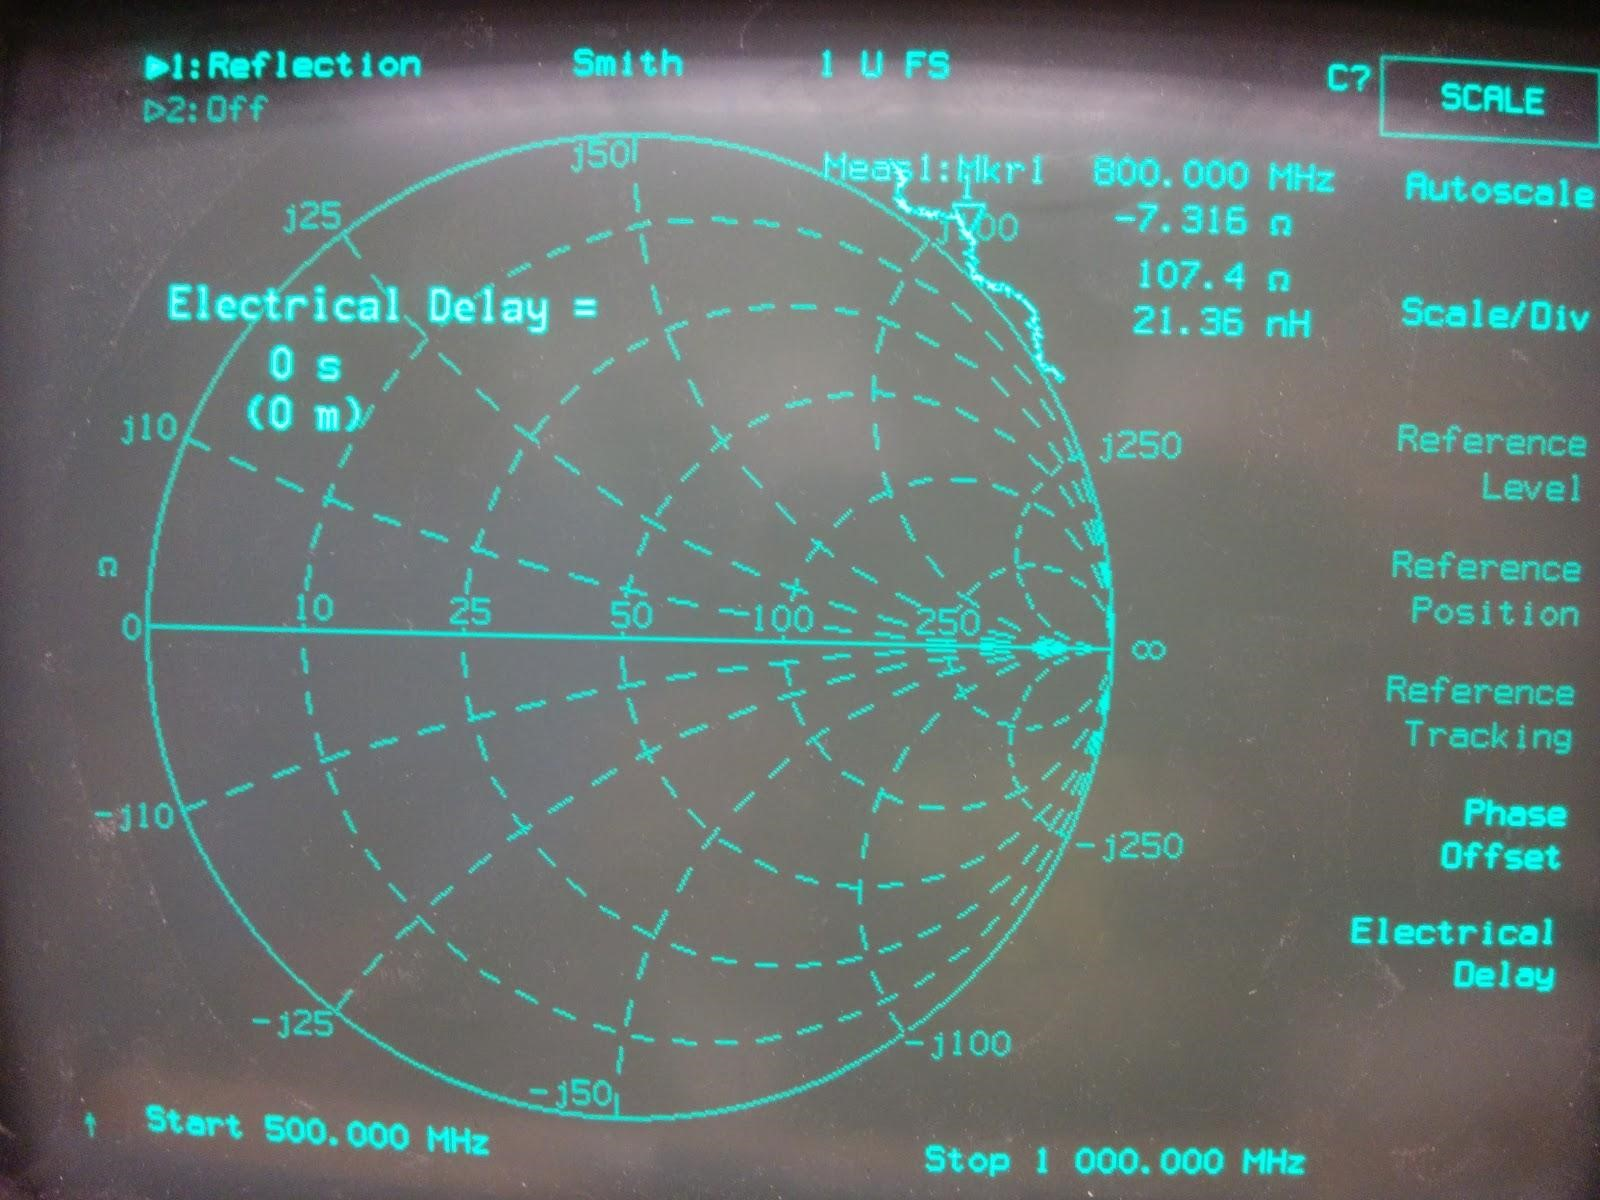
\includegraphics[width=0.8\textwidth]{./Images/252lossless.jpg}
    \caption{Network Analyzer response for a lossless line}
\end{figure}
\begin{figure}[H]
    \centering
    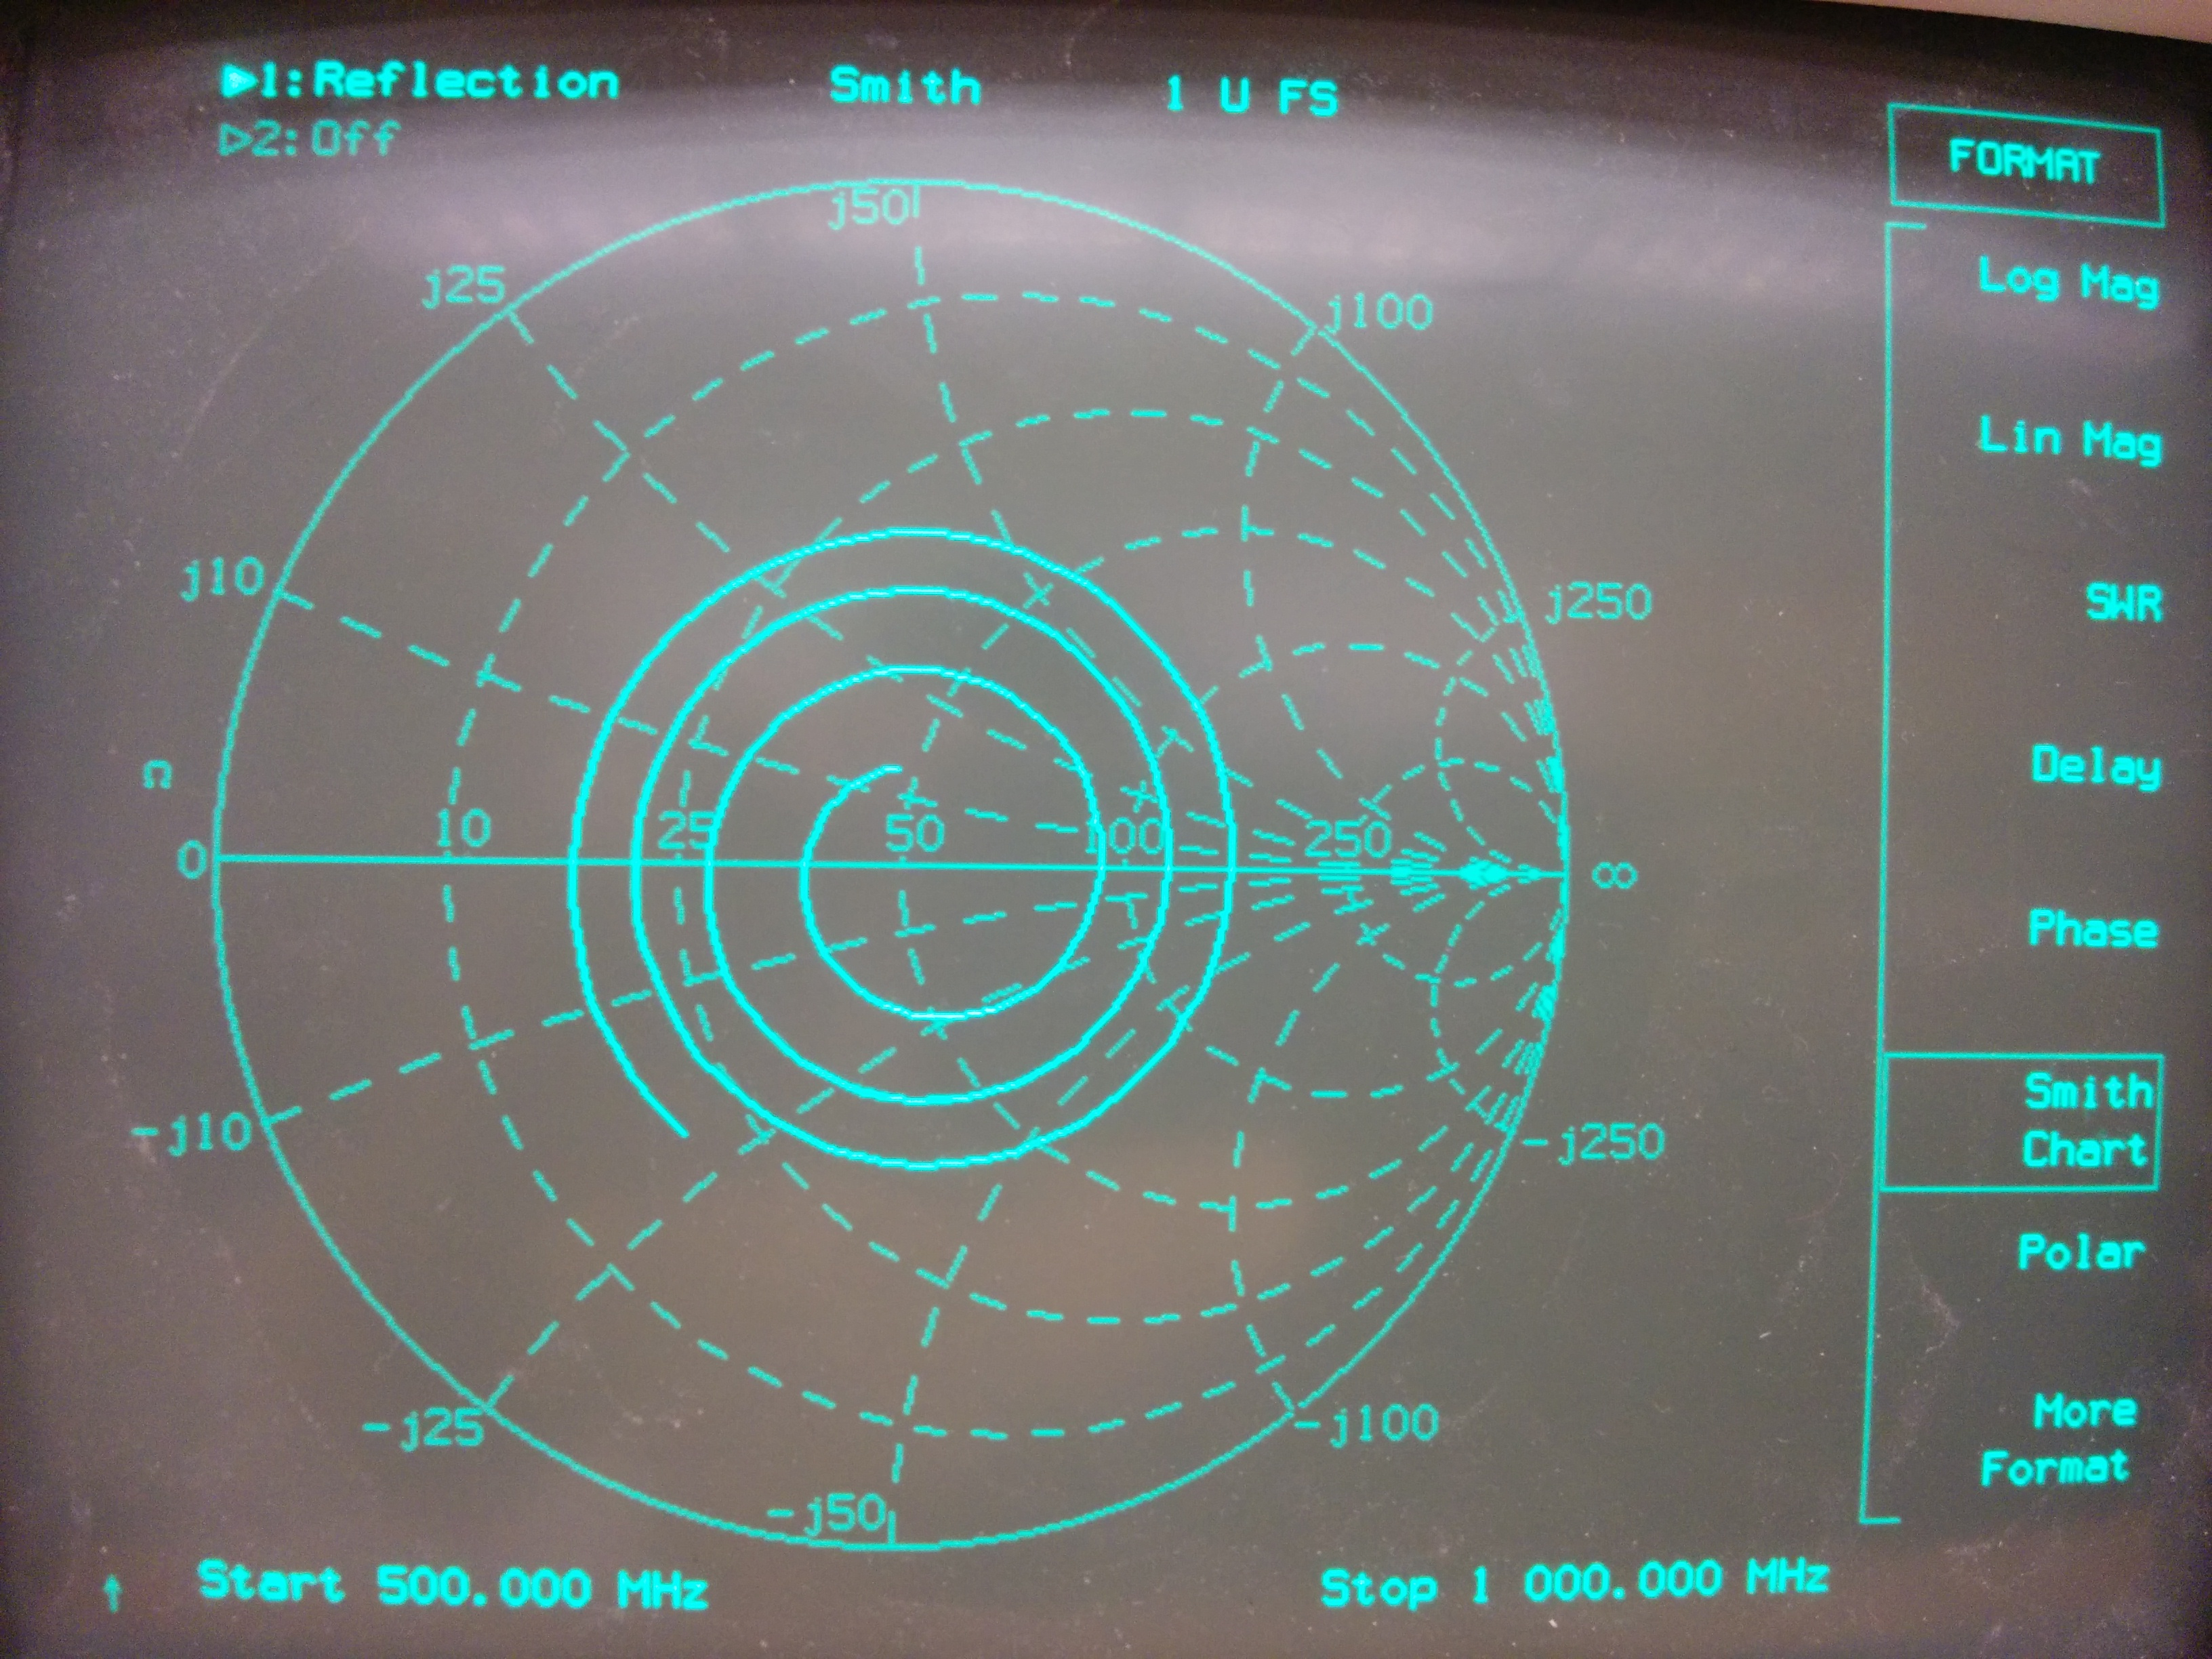
\includegraphics[width=0.8\textwidth]{./Images/252lossy.jpg}
    \caption{Network Analyzer response for a lossy line}
\end{figure}
\begin{figure}[H]
    \centering
    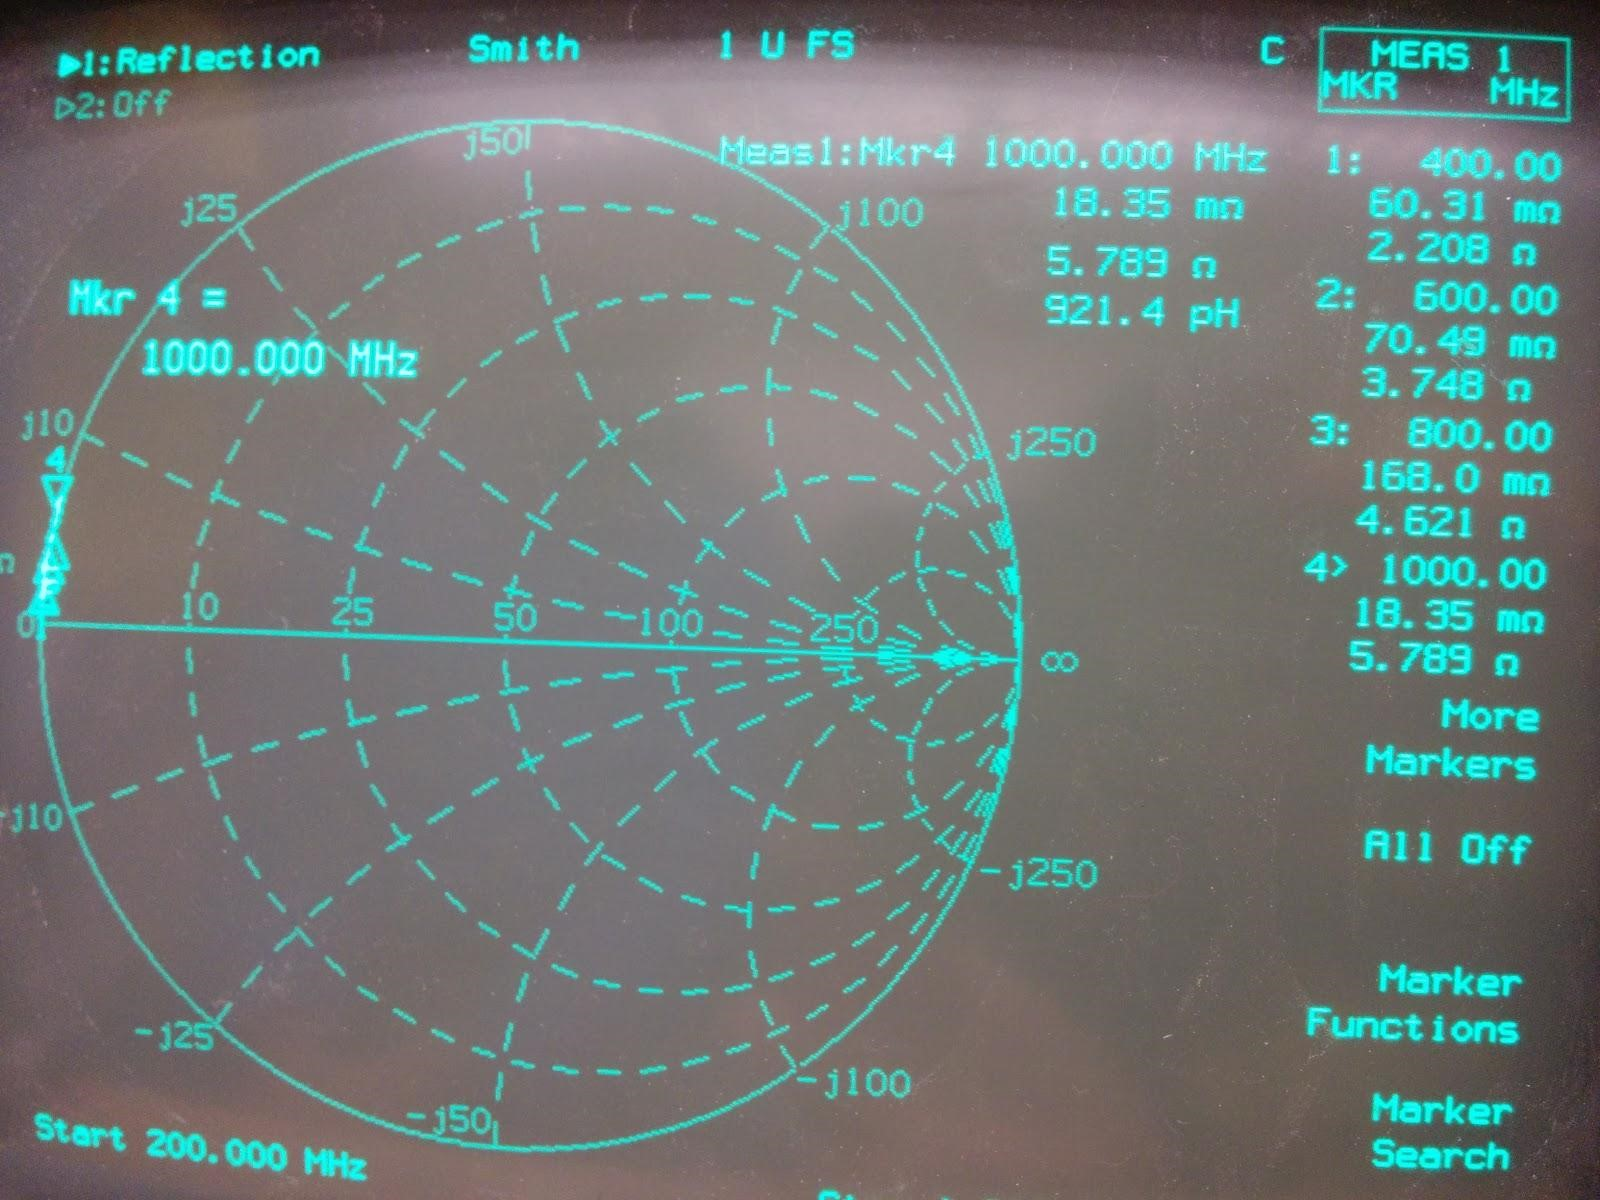
\includegraphics[width=0.8\textwidth]{./Images/253short.jpg}
    \caption{Network Analyzer response for a shorted load}
\end{figure}
\begin{figure}[H]
    \centering
    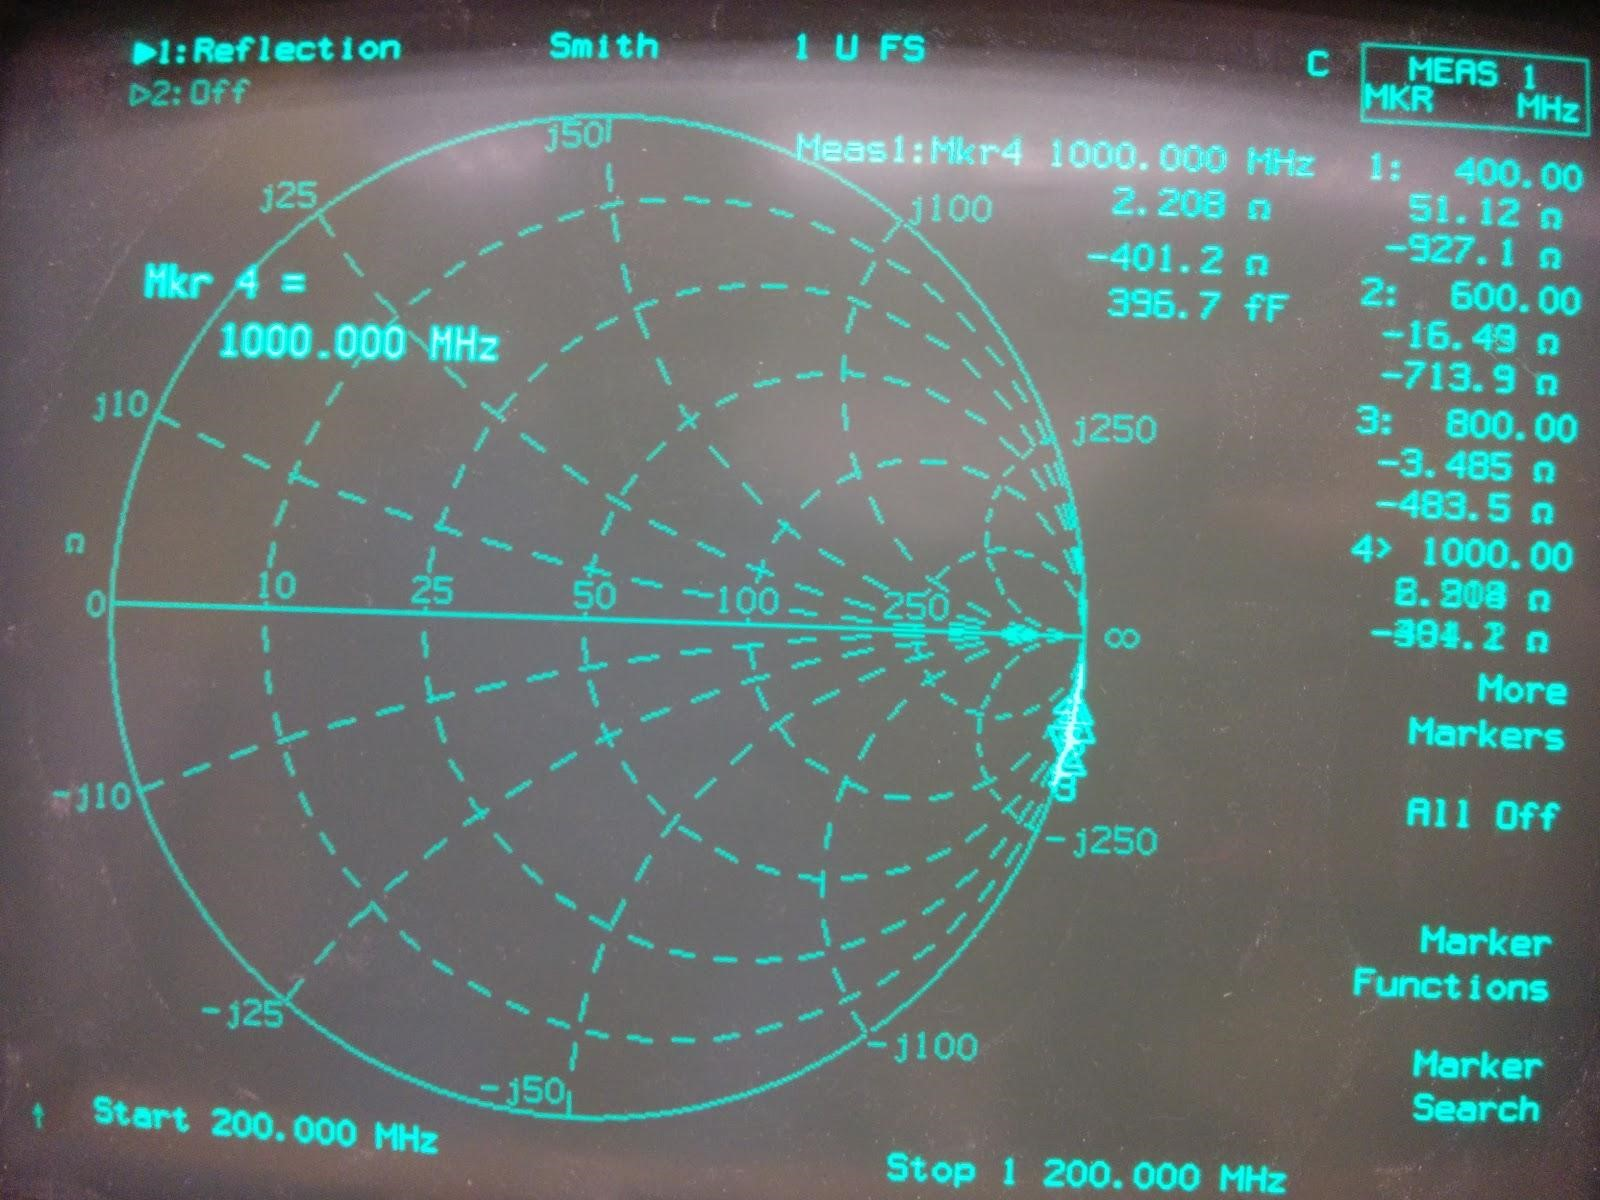
\includegraphics[width=0.8\textwidth]{./Images/253open.jpg}
    \caption{Network Analyzer response for an open load}
\end{figure}
\begin{figure}[H]
    \centering
    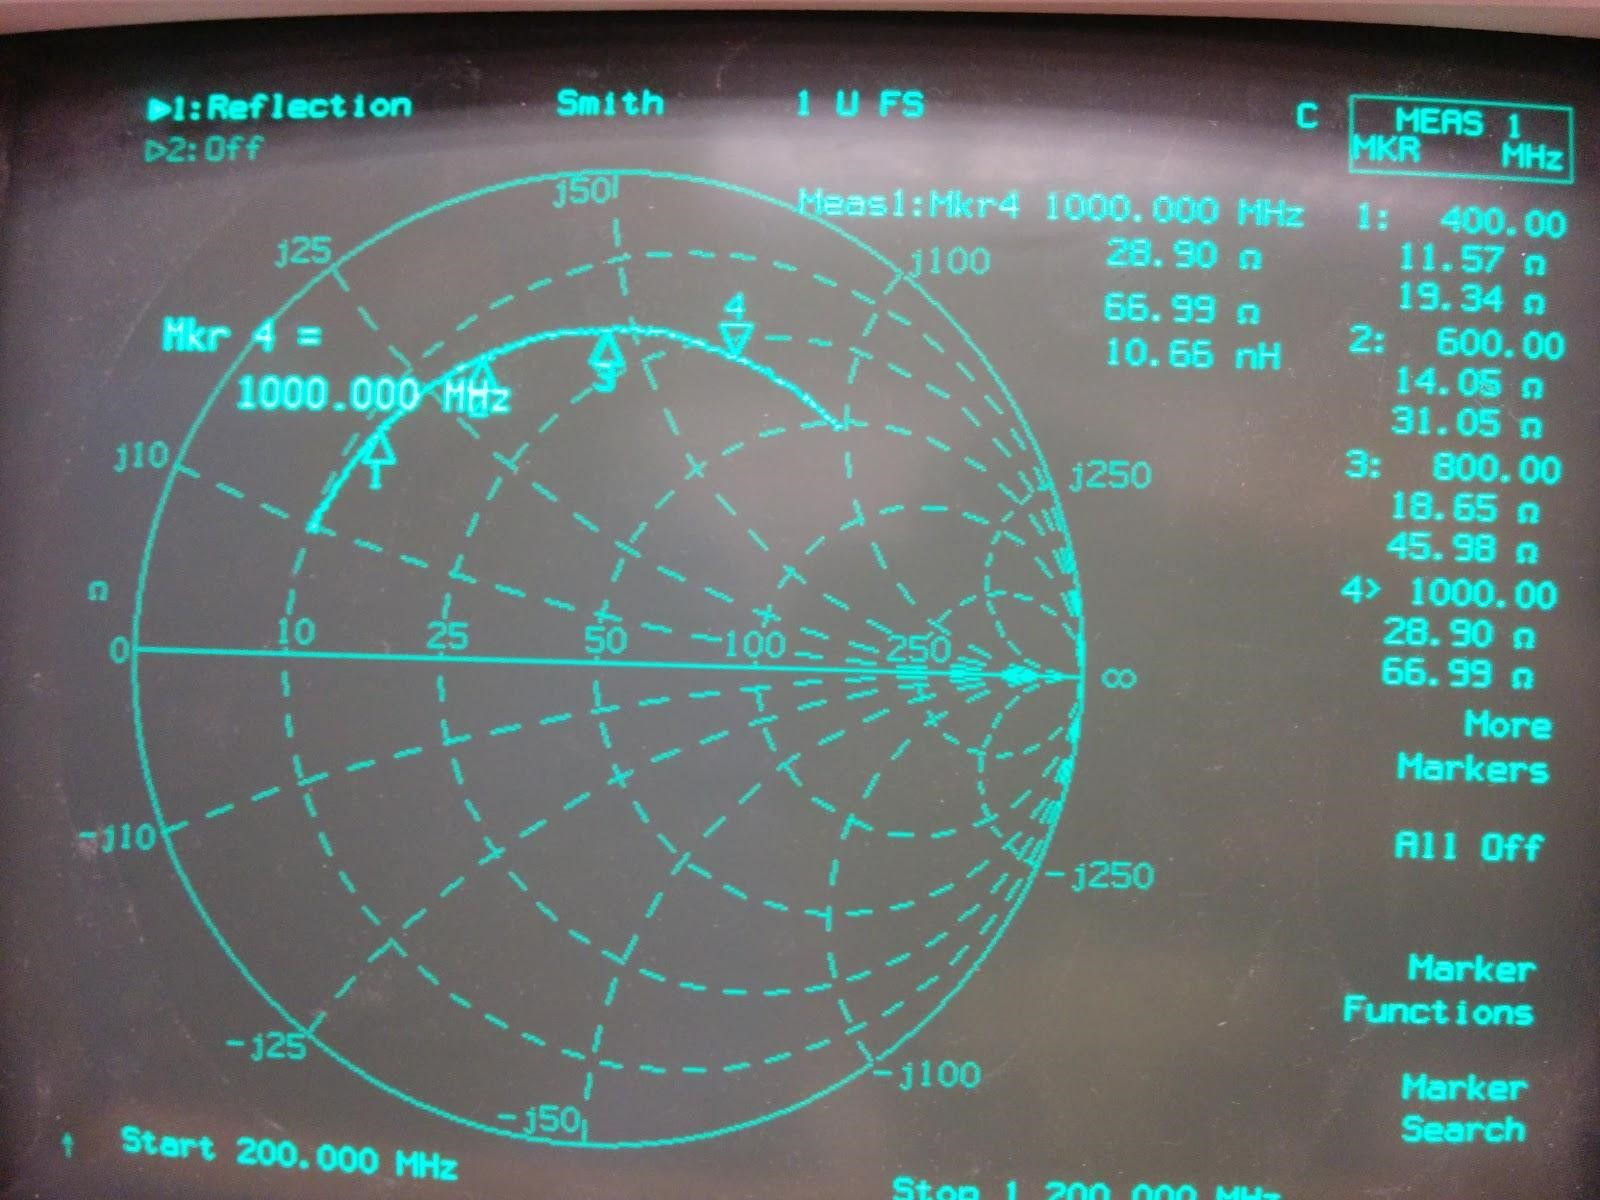
\includegraphics[width=0.8\textwidth]{./Images/253resisitive.jpg}
    \caption{Network Analyzer response for a resistive load}
\end{figure}
\begin{figure}[H]
    \centering
    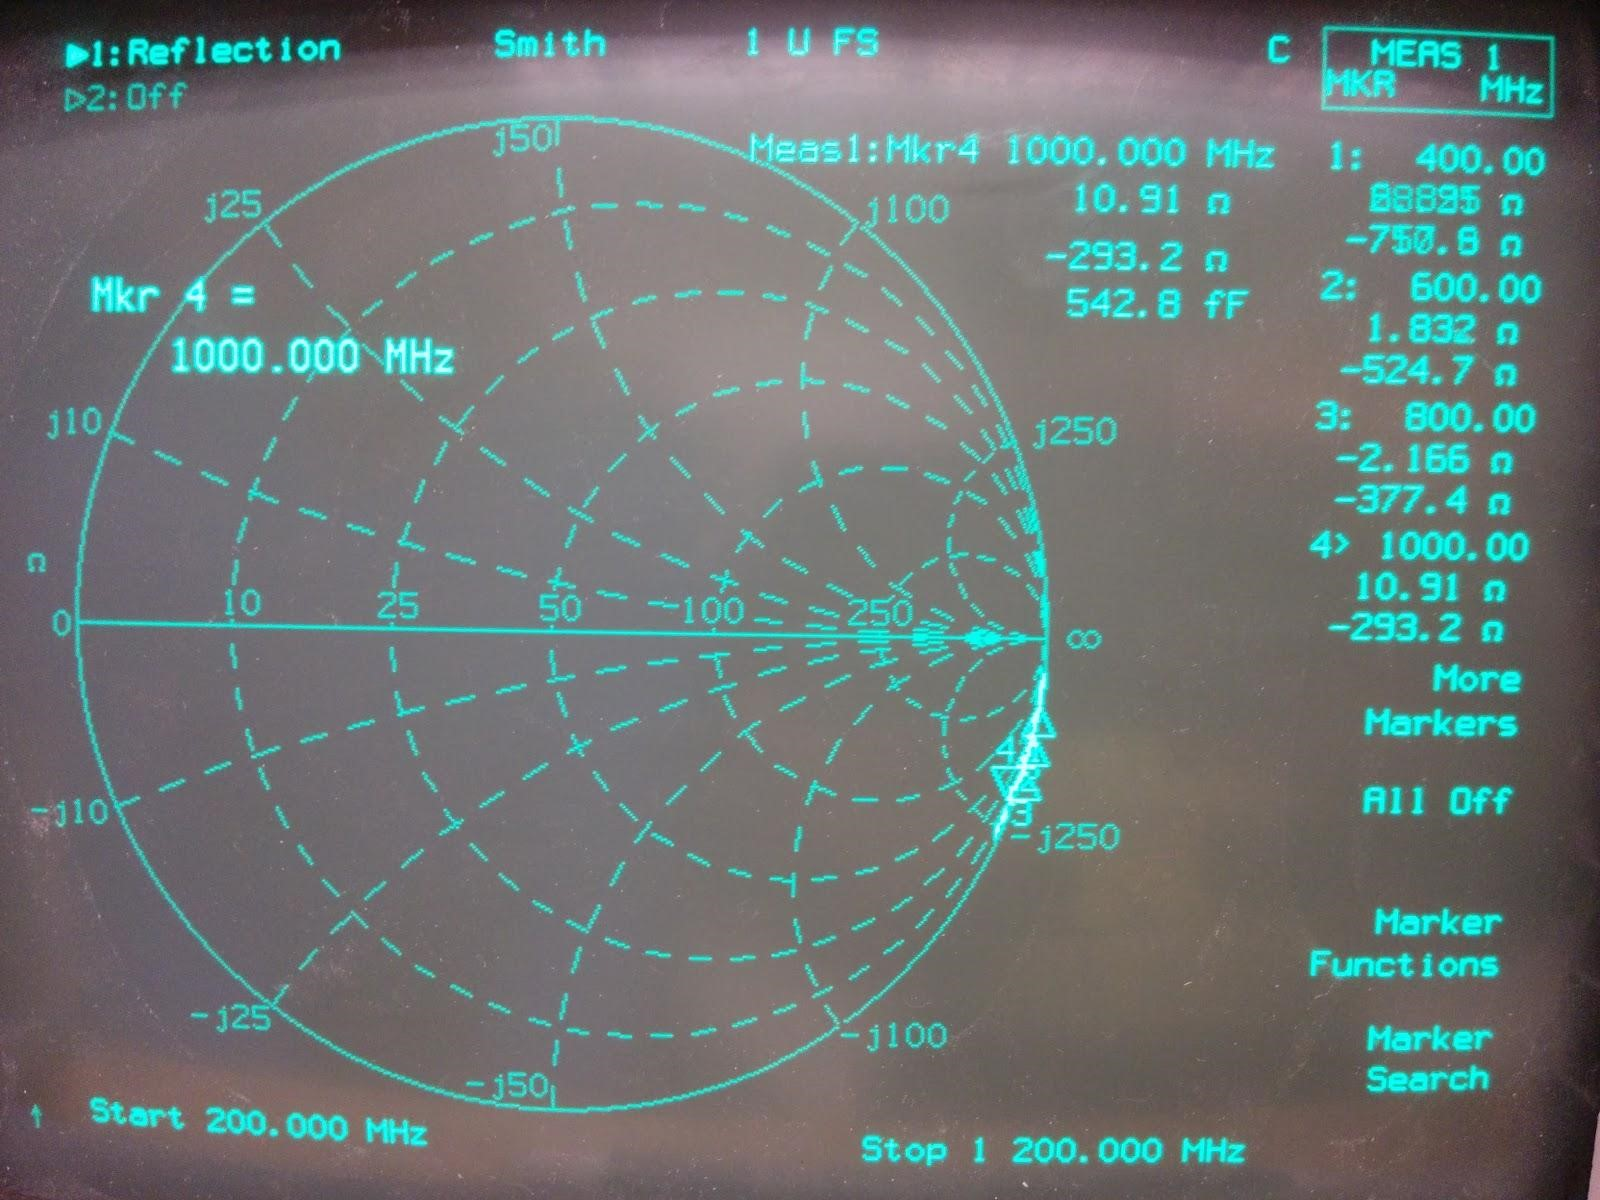
\includegraphics[width=0.8\textwidth]{./Images/253capacitive.jpg}
    \caption{Network Analyzer response for a capacitive load}
\end{figure}
\begin{figure}[H]
    \centering
    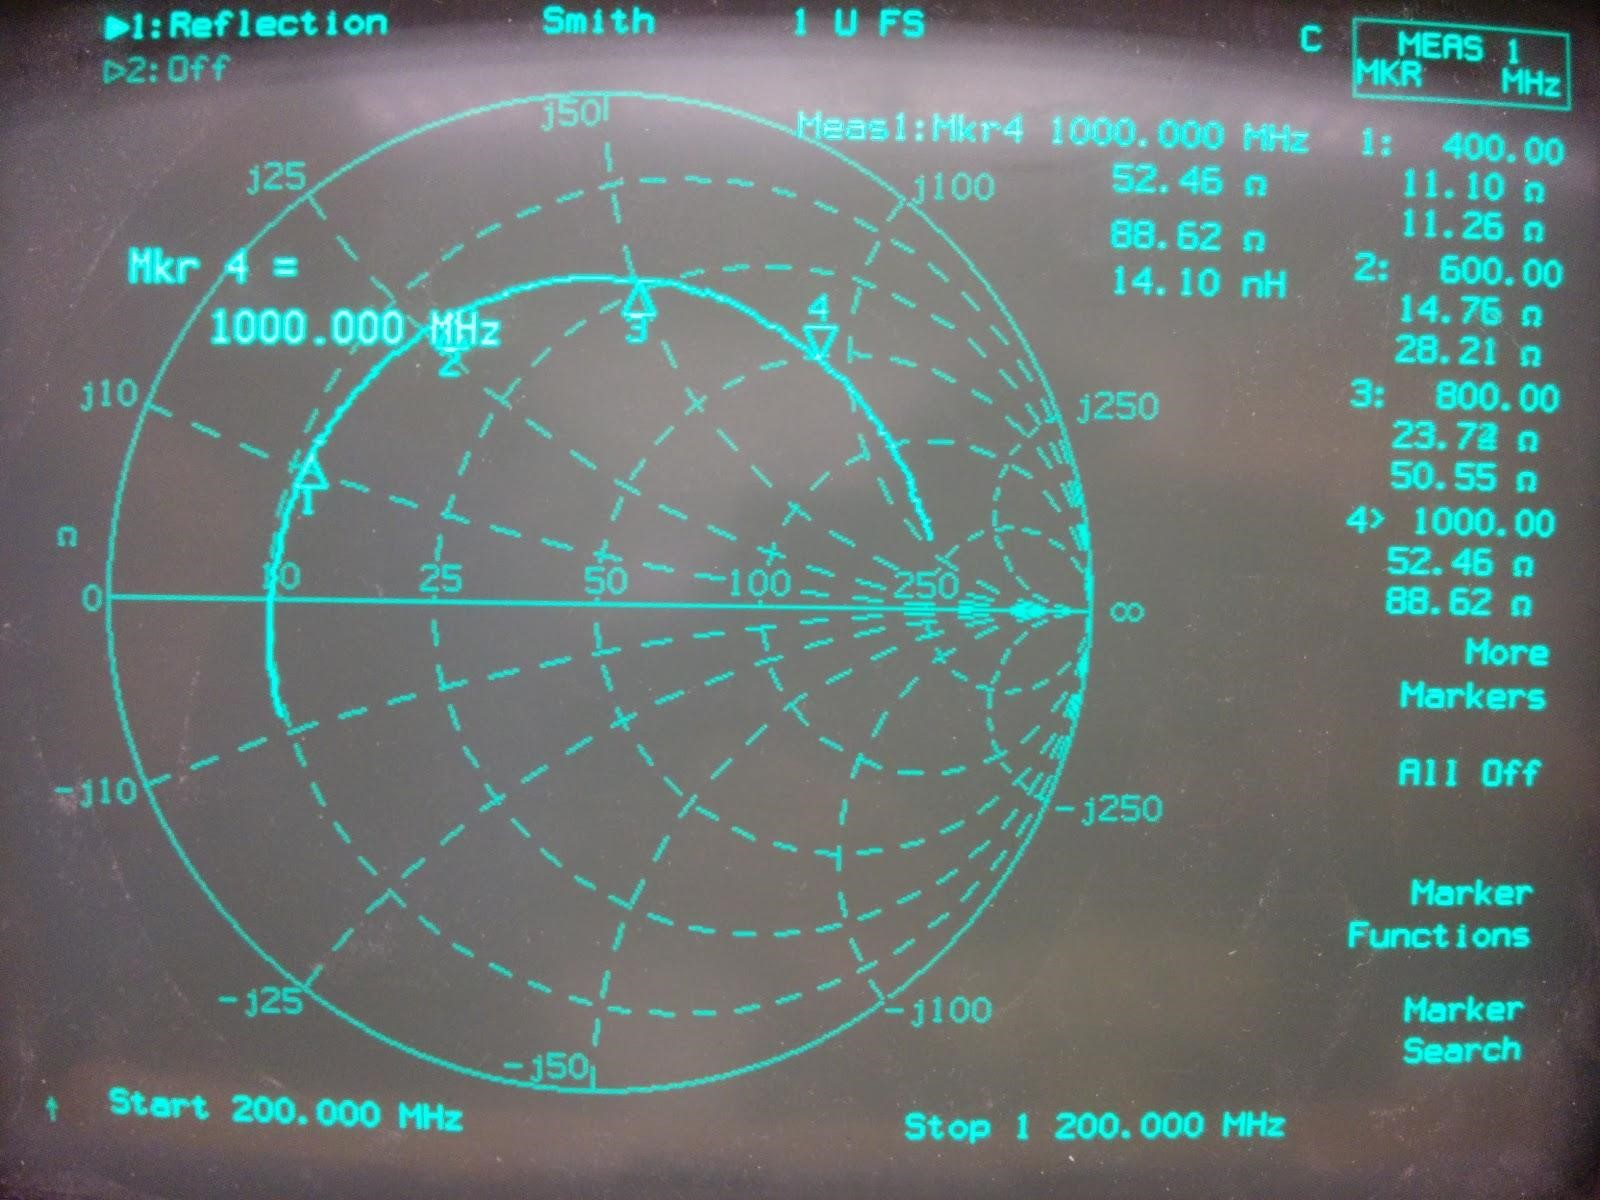
\includegraphics[width=0.8\textwidth]{./Images/253series.jpg}
    \caption{Network Analyzer response for a series load}
\end{figure}
\begin{figure}[H]
    \centering
    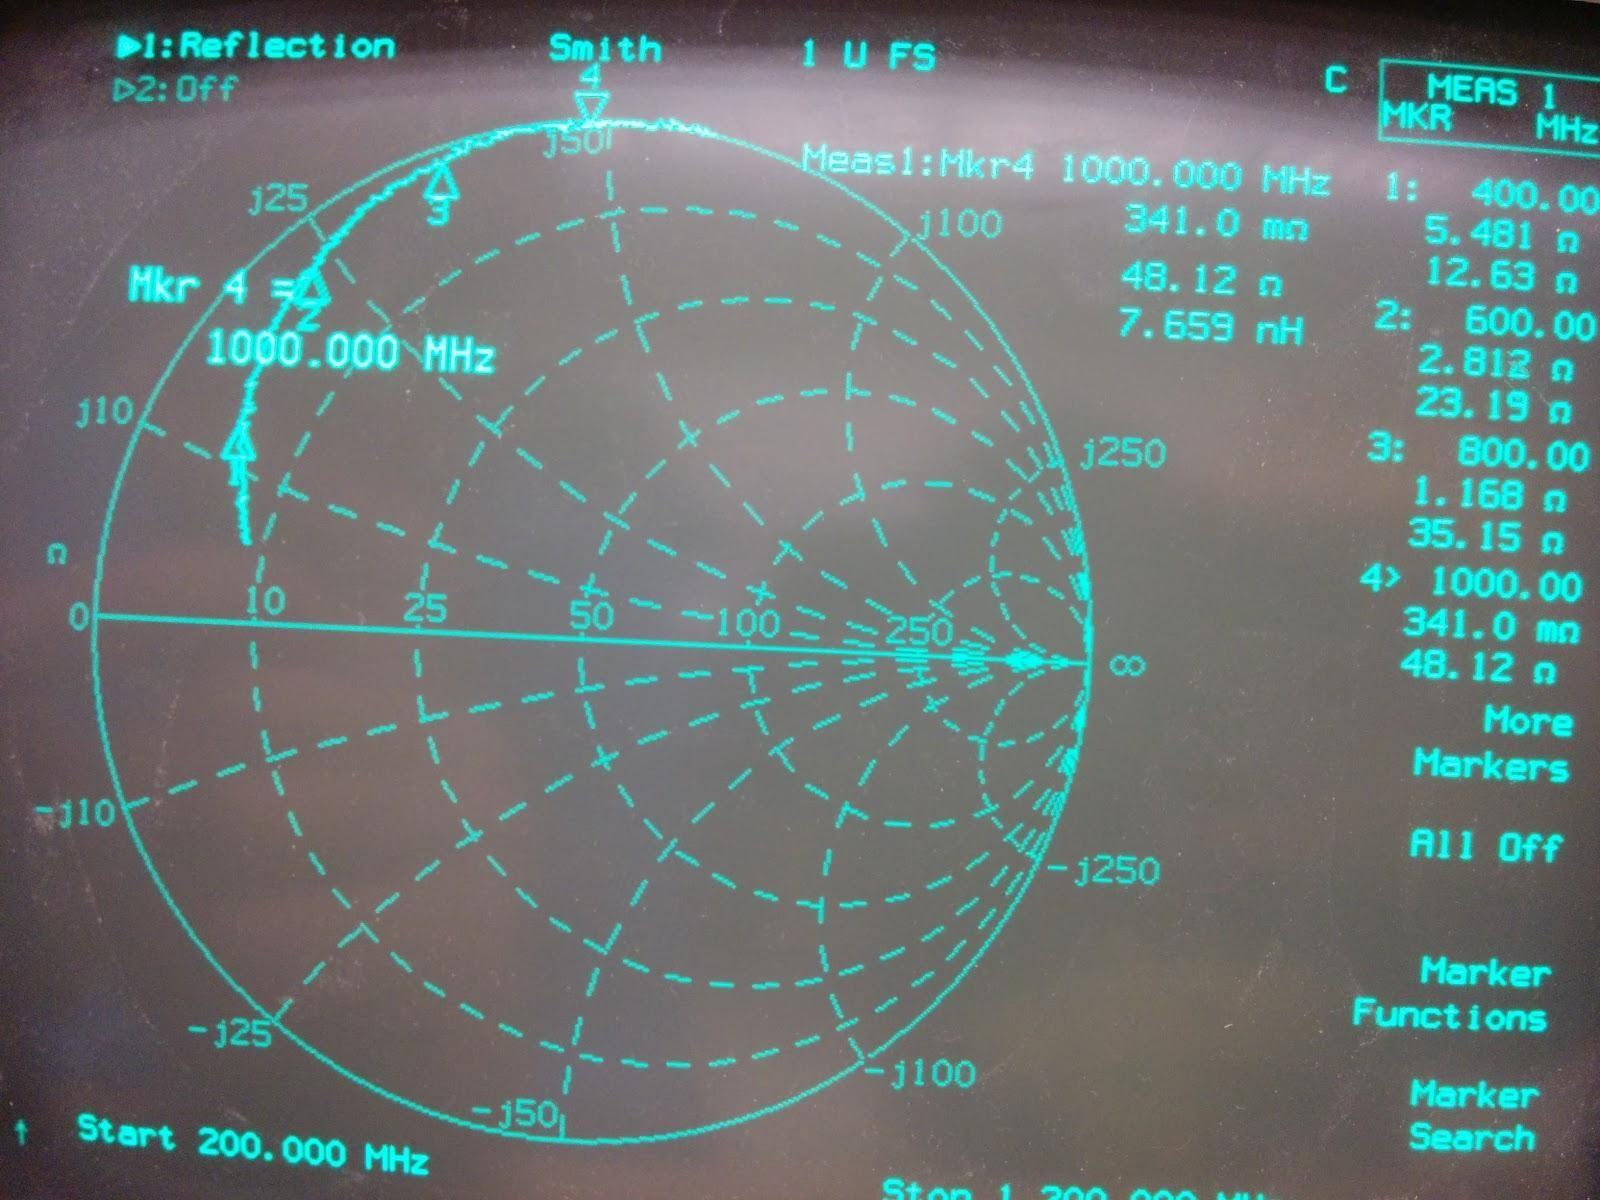
\includegraphics[width=0.8\textwidth]{./Images/253parallel.jpg}
    \caption{Network Analyzer response for a parallel load}
\end{figure}
\begin{figure}[H]
    \centering
    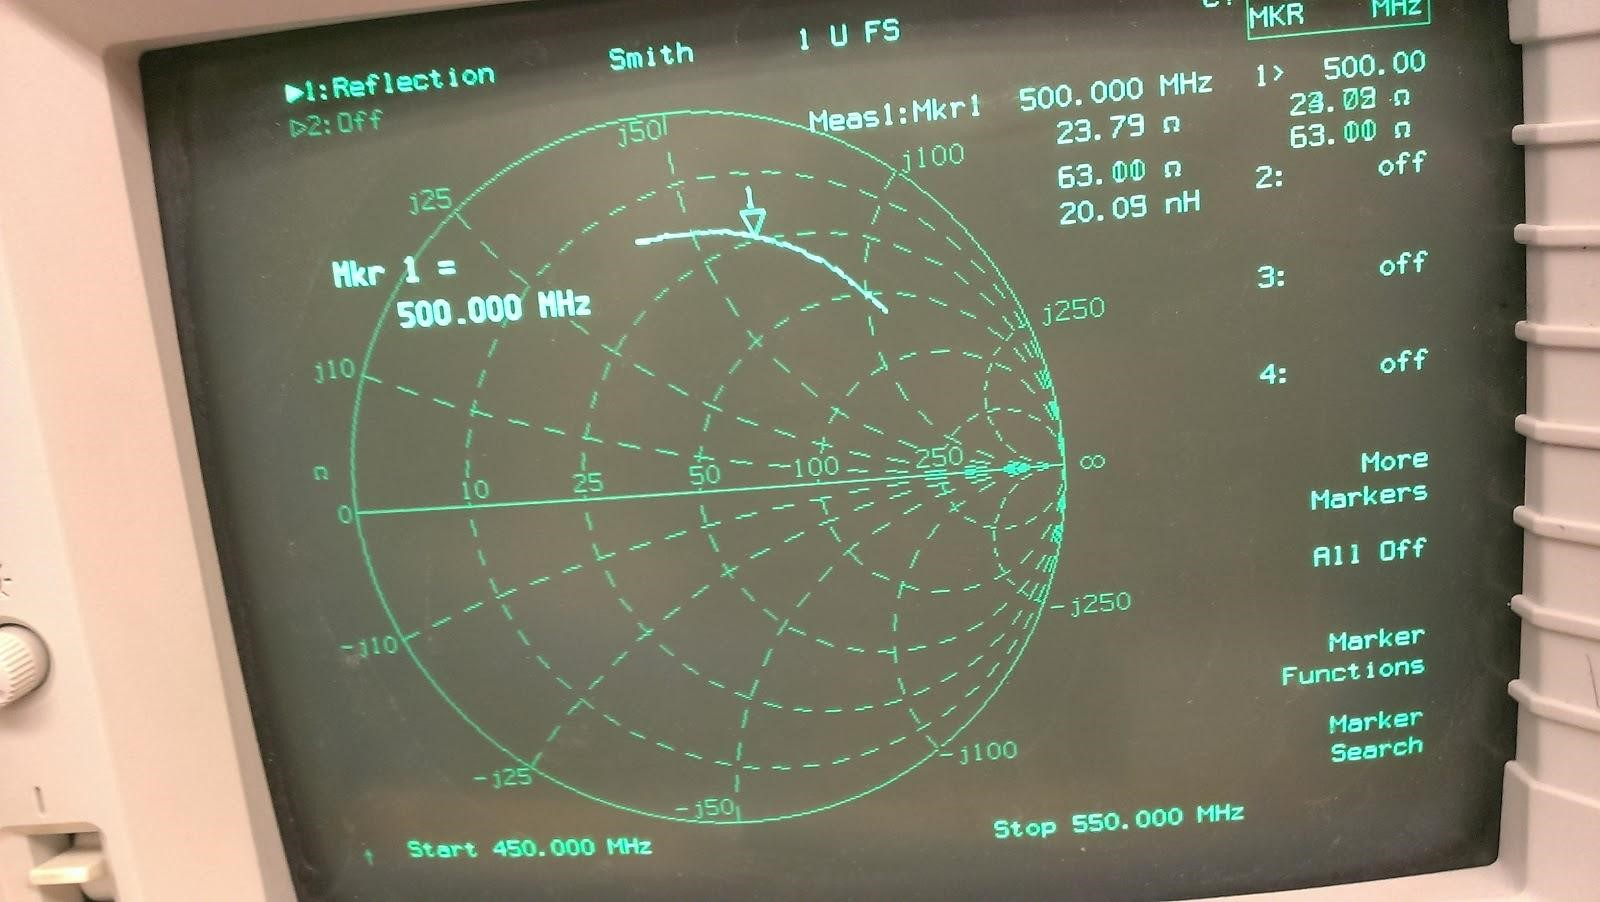
\includegraphics[width=0.8\textwidth]{./Images/254noadj.jpg}
    \caption{Network Analyzer response for the unmatched load}
\end{figure}
\begin{figure}[H]
    \centering
    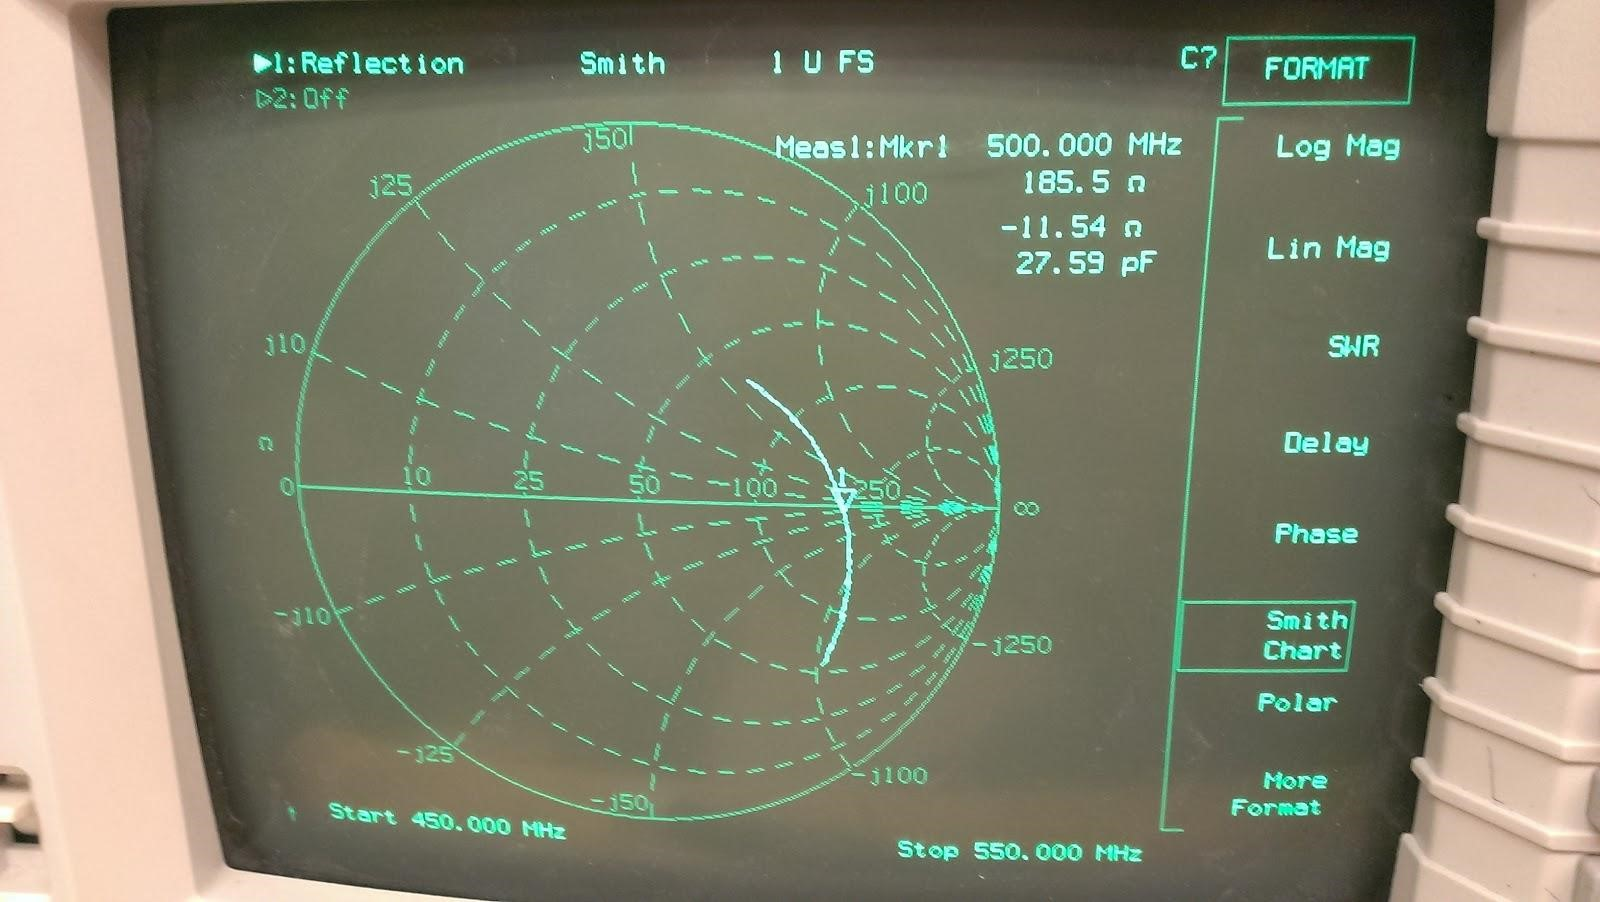
\includegraphics[width=0.8\textwidth]{./Images/254adj.jpg}
    \caption{Network Analyzer response for the matched load with the shorted stub}
\end{figure}
\end{document}